\documentclass{article}
\usepackage[utf8]{inputenc}
\usepackage{tikz}
\usepackage{standalone}
\usepackage{amsmath}
\usepackage{amsfonts}
\usepackage[a4paper, total={6in, 9in}]{geometry}



\newcommand{\Norm}{\mathcal{N}}
\newcommand{\Loss}{\mathcal{L}}
\newcommand{\R}{\mathbb{R}}
\newcommand{\bt}{\mathbf{t}}
\newcommand{\bU}{\mathbb{U}}
\newcommand{\bX}{\mathbf{X}}
\newcommand{\bx}{\mathbf{x}}
\newcommand{\by}{\mathbf{y}}
\newcommand{\bZ}{\mathbf{Z}}
\newcommand{\bz}{\mathbf{z}}

\newcommand{\parfrac}[2]{\frac{\partial #1}{\partial#2}}

\title{Causal Effect Inference using Normalising Flows - background research}
\author{Micha de Groot}
\date

\begin{document}
\maketitle

\section{Background research}

\subsection{causal inference, interventions, do-calculus and counterfactual reasoning}
The dominant research in artificial intelligence is all data-driven and broadly speaking looking for patterns in said data. The patters that most common AI models uncover are correlations between certain features in the data. In may problems this is a powerful tool that can perform a abundance of tasks, such as classification of images, translation of text or even the generation of new music. However, there is an inherent limit to models that can only uncover correlations: they can't find causal relation. Every class in statistics starts with the phrase: "Correlation is not causation." This mantra tells us that we should never interpret a correlation between a variable $A$ and variable $B$ as $A$ causes $B$. This is very much true, but sometimes we do like to know: does $A$ cause $B$? To answer such questions we need causal inference. 

In the causal inference framework, devised largely by Judea Pearl\cite{pearl1995causal} \cite{pearl2009causal}, we go beyond correlations by modelling the direction of cause and effect as well. This is done with Directed Acyclic Graphs (DAG); an example is given in Figure \ref{fig:graph_correlations_A_B}. Combined with structural equations for each edge in the graph, these form a Structural Causal Model. The parameters of these structural equations are similar to correlation coefficients except that the functions in which they are used have a clear direction. The estimation of such functions is what's called causal inference. 

\begin{figure}
    \centering
    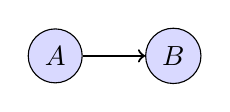
\begin{tikzpicture}
        \node[draw=black, circle, fill=blue!15!white] (a) at (0, 0) {$A$};
        \node[draw=black, circle, fill=blue!15!white] (b)at (1.5, 0) {$B$};
        \draw[->, thick] (a) -- (b);
    \end{tikzpicture}
    \qquad
    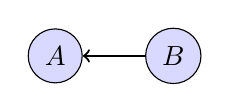
\begin{tikzpicture}
        \node[draw=black, circle, fill=blue!15!white] (a) at (0, 0) {$A$};
        \node[draw=black, circle, fill=blue!15!white] (b)at (1.5, 0) {$B$};
        \draw[->, thick] (b) -- (a);
    \end{tikzpicture}
    \qquad
    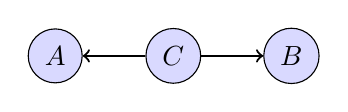
\begin{tikzpicture}
        \node[draw=black, circle, fill=blue!15!white] (a) at (0, 0) {$A$};
        \node[draw=black, circle, fill=blue!15!white] (b) at (3, 0) {$B$};
        \node[draw=black, circle, fill=blue!15!white] (c) at (1.5, 0) {$C$};
        \draw[->, thick] (c) -- (b);
        \draw[->, thick] (c) -- (a);
    \end{tikzpicture}
    \caption{Three possible DAGs for when $A$ and $B$ are correlated. On the left hand side $A$ causes $B$, in the middle $B$ causes $A$ and on the right hand side both $A$ and $B$ are caused by a third variable $C$.}
    \label{fig:graph_correlations_A_B}
\end{figure}

The reason we want to know the structure of these graphs and their corresponding functions is to answer causal questions. Although some cause and effect relations might seem deterministic, they are usually framed in a statistical fashion. This makes it possible to relate it to statistics and correlations, and in some cases even rephrase a causal question as a mere statistical one. The most important component in that regard is the \textit{do}-operator, see Equation \ref{equation:do_operation}. This equation tells us the probability of $A$ if we were to \textit{set} $B$ to a specific value; This is the causal effect from $B$ on $A$ in a probabilistic framing. The $pa_{B}$ is this equation indicates the set of all parents of $B$ in the causal graph, and if they are also parents of $A$ they are called confounders of $A$ and $B$. This immediately shows that we have to have knowledge of the causal graph to quantify a causal effect. For clarity  Equation \ref{equation:do_operation} also shows the conditional probability of $A$ given $B$ if we were to factor out the other parents of $A$. These two equations reduce to the same in certain cases, such as when $A$ has no parents, or when $B$ is the only parent of $A$. 
%Convince yourself that this is the case by looking back at Figure \ref{fig:graph_correlations_A_B}.

\begin{align}\label{equation:do_operation}
    p(A | do(B)) &= \int_{pa_B} p(A | B, pa_{B}) p(pa_{B}) \text{d} pa_B\\
    p(A | B) &= \int_{pa_B} p(A | B, pa_{B}) p(pa_{B}|B) \text{d} pa_B
\end{align}

Now the question arises: why is causal inference then perceived to be such a difficult problem if we can just slightly adjust an existing equation for computing conditional probabilities? This is because we either don't know the structure of the graph at all or if we can't observe certain confounders in the graph, called \textit{latent} confounders. If we don't know the graph we have to resort to causal discovery, which is beyond the scope of this research. If we do know the structure of the graph, or have strong indications to assume a certain structure, we can resort to methods to estimate the structural equations, even if not all variables are observed. The rest of this section will cover the existing work on causal inference in the case where there is a latent confounder.


% After that we will at some point talk about do-calculus and how you can measure a causal effect if you know the graph. Backdoor adjustment. Something about assuming a graph structure.

% Existing work on causal inference that doesn't use deep learning




\subsubsection*{Distinguishing cause from effect using observational data: methods and benchmarks}
--Book (chapter)\cite{mooij2016distinguishing}, quite long, will look for useful info--

Causal discovery in the bivariate case has been mostly based on the difference in complexity of the factorisation of the joint distribution $p(X,Y)$. If $p(X)p(Y|X)$ consists of two simpler distributions than $p(Y)p(X|Y)$ then it is likely that $X$ is a cause of $Y$ instead of the other way around. The chapter discusses several extensive benchmarks for these types of tests.

Another definition for "$X$ is a cause of $Y$" is that $p(Y|do(X=x)) \neq p(Y|do(X=x'))$




\begin{figure}
    \centering
    \includestandalone{Figures/causal_graph_one_proxy_one_confounder}
    \caption{Causal graph with one proxy variable. $\bt$ is the variable we intervene on; $\by$ is the outcome; $\bZ$ is the latent confounder; and $\bX$ is the observed proxy variable.}
    \label{fig:causal_graph}
\end{figure}
\subsection{Deep learning and Generative modelling}

\subsubsection*{Autoencoding Variational Bayes}
The problem of finding the posterior distribution of the latent variable of data is a problem that has been approached with different methods. Variational Inference is one of such methods, which has become very popular through the Variational Autoencoder(VAE) \cite{kingma2013auto}. The VAE is a framework that uses the principle of a variational distribution to approximate the posterior distribution. By using neural networks to parameterise the variational distribution and the likelihood, and the reparameterisation trick, it is possible to learn the variational distribution and the data likelihood through gradient descent methods. Because of the positioning of the VAE within the deep learning it was able to distinguish itself from other variational inference methods. 

Although the VAE has been used successfully for variational inference, it does have its limits. A requirement for a VAE is that the variational distribution is a parameterised distribution that is chosen beforehand, usually a Gaussian with diagonal covariance. This of course limits the model in capturing more complex posterior distributions. Another disadvantage is that the likelihood tends to converge to a per-feature mean. This means that in datasets where individual features are either multimodal or are far from the mean, given a specific value of the latent value, the likelihood is fitted poorly on the data. This is apparent in image-based datasets. The images sampled from the model tend to be very blurry and lack sharp edges.

\subsubsection*{Variational Inference with Normalising Flows}
A normalising flows is a type of model that is capable of variational inference. Is is able to learn flexible, arbitrarily complex and scalable approximate posterior distributions. The main advantage it has over the VAE is that the approximation of the posterior is not limited to parameterised distributions. The idea is to start with a simple initial density that is parameterised, and transforming that into an arbitrary complex distribution by applying a series of invertible transformations. The final probability density is defined by applying the change of variable formula to the density of the original simple distribution. The only requirement of the invertible mapping is that its Jacobian has to be efficiently computed, as it has to be evaluated many times, both during training and testing.

The basis lies in the original negative free energy function derived from introducing the approximate posterior distribution in the marginal log likelihood:

\begin{equation}\label{equation:neg_free_energy}
    \begin{split}
    \log p_\theta(\bx) &= \log \int p_\theta(\bx | \bz) p(\bz) d\bz\\
    &= \log \int \frac{q_\phi(\bz|\bx)}{q_\phi(\bz|\bx)} p_\theta(\bx | \bz) p(\bz) d\bz\\
    &\geq -\mathbb{D}_{KL}[q_\phi(\bz|\bx) || p(\bz)] + \mathbb{E}_q[\log p_\theta(\bx|\bz)] = -\mathcal{F}(\bx)
    \end{split}    
\end{equation}
The negative free energy function $\mathcal{F}$ is also known as the Evidence Lower Bound(ELBO). The novelty of normalising flows lies in how the approximate posterior $q_\phi(\bz|\bx)$ is defined.  


\subsubsection*{Analyzing Inverse Problems with Invertible Neural Networks}
The invertibility of flow-based models makes them suitable for recovering posterior information of complex physical systems. This has been proposed by Ardizzone et al. \cite{ardizzone2018analyzing} in the form of Invertible Neural Networks. Given some process $\bx \rightarrow \by$ with observed $\by$ and unobserved $\bx$ oe would like to know how to recover $\bx$ for a ceartain $\by$. This is done by using an approach based on the RealNVP\cite{dinh2016density} model. Since the forward process has inherent information loss, a latent variable $\bz$ is introduced that captures the information in $\bx$ that is not contained in $\by$, turning the process into $f(\bx) = [\by, \bz]$  and $\bx = f^{-1}(\by, \bz) = g(\by, \bz)$. Because of the nature of Normalising-Flow models, $g(\by, \bz)$ does not have to be modelled separately. The density $p(\bz)$ is shaped as a Gaussian. 

This differs from the causal graph in Figure \ref{fig:causal_graph} because both $\bx$ and $\bz$ are unobserved. Though the INN approach might still be useful if we were to recover $\bZ$ from a given $\bX$. I think this would be an approximation for $p(\bZ | \bX)$, which could then be used to approximate equation \ref{equation:intervention}. 


\subsubsection*{Density estimation using Real-NVP}
Real NVP: \cite{dinh2016density}

\subsubsection*{Sylvester Normalising Flows for Variational Inference}
Sylvester Flow: \cite{berg2018sylvester}


\subsection{Intersection of generative modelling and causal inference}

\subsubsection*{Causal Effect Inference with Deep Latent-Variable models}
The paper by Louizos et al.\cite{louizos2017causal} serves as a good starting point for research into the use of Normalising Flows in causal inference. It explores the possibility of measuring the direct effect of one observed variable on another given that there is a shared unobserved confounder by using a proxy variable that has the same confounder. This causal graph is shown in Figure \ref{fig:causal_graph}. Their contribution is doing this task by using Variational Autoencoders\cite{kingma2013auto} to recover the Individual Treatment Effect(ITE):
\begin{equation}\label{equation:ITE}
    ITE(x) := \mathbb{E}[\by | \bX = x, do(\bt = 1)] - \mathbb{E}[\by | \bX = x, do(\bt=0)]
\end{equation}

\noindent
The paper states that $\bt$ does not have to be binary for their approach to work but it is assumed for simplicity and compatibility with prior benchmarks. First the joint distribution $p(\bZ, \bX, \by, \bt)$ is approximated with a VAE that consists of several neural networks. With that $p(\by | \bX, do(\bt=1))$ can be identified:

\begin{equation}\label{equation:intervention}
    \begin{split}
    p(\by | \bX, do(\bt=1)) &= \int_\bZ p(\by | \bX, do(\bt=1, \bZ)) p(\bZ | \bX, do(\bt = 1)) d\bZ \\
                            &= \int_\bZ p(\by | \bX, \bt = 1, \bZ) p(\bZ | \bX) d\bZ
    \end{split}
\end{equation}

\noindent
The inference network captures $q(\by | \bt , \bX), q(\bZ | \bt, \by, \bX), q(\bZ| \bt, \by, \bX)$ and the generative network captures $p(\bX | \bZ), p(\bt | \bZ), p(\by | \bt, \bZ)$. These are then used to compute a sample average for the ITE.

The problem with trying to translate this to Normalising-Flow model is that an NF model cannot simply model conditional distributions. For this we would require a way to model arbitrary Bayesian networks with NF. 


\subsubsection*{CausalGAN: Learning Causal Implicit Generative Models with Adversarial Training}
CausalGAN: \cite{kocaoglu2017causalgan}.

\subsubsection*{A Meta-Transfer Objective for Learning to Disentangle Causal Mechanisms}
Disentanglement with causality \cite{Bengio2020A}

\subsubsection*{Causal Confusion in Imitation Learning}
Causal confusion: \cite{de2019causal}

\subsubsection*{Causal Correct Partial Models for Reinforcement Learning}
Causally correct RL: \cite{rezende2020causally}

% \section{Possible research directions}
% \subsubsection*{More complex graphs}
% In the reviews of \cite{louizos2017causal} it is mentioned that it might be interesting to look at more complex causal graphs with more proxy variables such as those discussed in \cite{miao2018identifying}. From what I gathered these other setups with confounders are more specific instances of the problem and the graph in figure \ref{fig:causal_graph} is the most general case. 

% \subsubsection*{Causal graph discovery with NF}
% Complex problem. Solved for small number of variables. In the simplest form we are examining if $p(x) = p(x|y)$ or $p(x) \neq p(x|y)$, which requires the modelling of conditional distributions.

% \subsubsection*{Improve on CEVAE with NF}
% Requires some way to mode conditional probabilities with NF. Has the possibility of increasing the lower bound.

% \section*{Possible designs of Normalising Flow}
% For now we focus on 
% \subsection{}
% \begin{equation}
%     p(\by | \bx, \bt) = \frac{p(\by, \bx, \bt)}{\sum_\by p(\by, \bx, \bt)}
% \end{equation}
% \begin{equation}
%     p(\by, \bx, \bt) = p(\bz) |J|
% \end{equation}
% \begin{equation}
%     p(\by | \bx, \bt) = \frac{p(\bz)|J|}{\sum_\by p(\bz)|J|}
% \end{equation}
% Simplest version. Probably not strong enough model. We can compute $\bz$ from the joint distribution of the other variables, but it isn't straightforward to me how we would sum over $\by$.

% \subsection{}
% Splitting $\bz$ into multiple variables might allow :
% \begin{align}
%     p(\bx, \bt, \by) &= p(\bx)p(\by|\bt)p(\bt)\\
%     p(\bx) &= p(\bz_x) |J|\\
%     p(\bt) &= p(\bz_t) |J|\\
%     p(\by| \bt) &= p(\bz_y|\bt) |J|\\
% \end{align}
% or
% \begin{align}
%     p(\bt, \by | \bx) &= p(\bt) p(\by | \bt, \bx)\\
%     p(\bt) &= p(\bz_t) |J|\\
%     p(\by | \bt, \bx) &= p(\bz_y) |J|
% \end{align}
% For either of these two to make sense there would have to be a common latent confounder for all $\bz$ variables, called $\bU$, which could be recovered from the $\bz$ variables in the same way that is done by Ardizzone et al. \cite{ardizzone2018analyzing}. We could then sample from $p(\bU)$, invert the flow to get $\bz_t$ and $\bz_x$. By then conditioning on $\bt$, $\bz_y$ can be obtained and form that $\by$. These two options are represented in Figure \ref{fig:causal_graph_split_confounder}.

% Problem here is that during training the "forward process", as it is called by \cite{ardizzone2018analyzing}, is known and can be used to sample an arbitrary amount of training data by sampling from the appropriate prior. Since we have no information on the real confounder, this is not really an option.

% \begin{figure}
%     \centering
%     \includestandalone{Figures/causal_graph_one_proxy_split_confounder}
%     \caption{Splitting the common confounder into multiple variables that have one shared confounder. The effect from $\bt$ can be passed through the new latent variable $\bz_y$ or not.}
%     \label{fig:causal_graph_split_confounder}
% \end{figure}


% We need a way to measure the effect of the confounder on $\by$ given $\bx$  and $\bt$. If we have some flow form $\bx, \by$ and $\bt$ to the confounder, we can't reverse it to get $\by$. One advantage is that $\bt$ is binary. This means we can just make two distributions, one for $\bt=1$ and one for $\bt=0$ 

% What if we do a sort of Monte Carlo approach where we have a flow from x, y, t to z and sample a bunch of y values and then sum/average the z values, we can then reverse the flow to get the real y?


% \newpage
% \subsection{Basic equations designing the setup}
% \subsubsection{Three flows}
% We make $\bZ$ an $N$ dimensional vector and define three flows. One from $\bx$ to $\bZ$. $\bx$ will be $M$ dimensional and the remaining $N-M$ dimensions will come form some auxiliary variable $\bZ_x$. 
% Next we have a flow from $\bZ$ to $\bt$ and $\bZ_t$. $\bt$ is one dimensional and binary, $\bZ_t$ will have $N-1$ dimensions. If we want to do an intervention, we could do that after this flow. The third flow is from $\bZ_t$ and $\bt$ to $\by$ and $\bZ_y$, where we have to define some split for the $N$ dimensions from the input. A graphical representation is given in Figure \ref{fig:flow_graph_three_flows}. The joint distribution over all variables under this model is defined as:
% \begin{equation}
%     p(\bx, \bt, \by, \bz) = p(\bx|\bz)p(\bt|\bz)p(\by|\bt, \bz)p(\bz)
% \end{equation}


% \begin{figure}
%     \centering
%     \includestandalone{Figures/flow_graph_3_flows}
%     \caption{Graphical representation of the flow model with three flows. With this model we can intervene on $\bt$ and the reverse flow can be initiated with only $\bx$.}
%     \label{fig:flow_graph_three_flows}
% \end{figure}

% \noindent
% The transitions in Figure \ref{fig:flow_graph_three_flows} will be modelled by the following set of equations:
% \begin{align}
%     [\bz, \bZ_x] = f_x(\bz)\quad &(=) \quad \bz = g_x(\bx, \bZ_x)\\
%     [\bt, \bz_t] = f_t(\bz)\quad &(=) \quad \bz = g_t(\bt, \bZ_t\\
%     [\by, \bZ_y] = f_y(\bt, \bZ_t)\quad &(=) \quad [\bt, \bZ_t] = g_y(\by, \bZ_y)
% \end{align}
% \noindent
% And the following set of probability distributions:
% \begin{align}
%     \bz \sim p(\bz) &= \Norm(\bz | 0, I)\\
%     \bZ_x \sim p(\bZ_x) &= \Norm(\bZ_x | 0, I)\\
%     \bZ_t \sim p(\bZ_t) &= \Norm(\bZ_t | 0, I)\\
%     \bZ_z \sim p(\bZ_z) &= \Norm(\bZ_z | 0, I)\\
%     q(\bx, \bZ_x) &= p(\bz) \left|\det\parfrac{f_x(\bz)}{\bz}\right|^{-1}\\
%     q(\bt, \bZ_t) &= p(\bz) \left|\det\parfrac{f_t(\bz)}{\bz}\right|^{-1}\\
%     q(\by, \bZ_y) &= p(\bz) \left|\det\parfrac{f_y(f_t(\bz))}{\bz}\right|^{-1}
% \end{align}

% \subsubsection{Two flows}
% For the second proposal most of the setup is kept the same. What changes is that $\bZ_x$ and $\bZ_t$ are merged into one random variable and the normalising flow $f_x$ and $f_t$ are merged into one flow. This result in $\bz \in \R^N, \bx \in \R^M, \bt \in R, \bZ_x \in \R^{N-M-1}$ and $[\bx, \bZ_x, \bt] = f_x(\bz)$. The flow to $\by$ is kept as $[\by, \bZ_y] = f_y(\bt, \bZ_x)$. 

% \begin{figure}
%     \centering
%     \includestandalone{Figures/flow_graph_2_flows}
%     \caption{Graphical representation of the flow model with two flows. With this model the dependence between $\bx$ and $\by, \bt$ is made explicit with the first flow from $\bz$.}
%     \label{fig:flow_graph_three_flows}
% \end{figure}

% \subsubsection{Comparison of the two model setups}
% First off I think the split into at least two normalising flows is unavoidable since we have to be able to generate $\bt$ from $\bz$ before we generate $\by$. This  immediately implies that the extra latent variable $\bZ_x$ or $\bZ_x$, depending on the version, is required a well. Otherwise the information flowing from $\bz$ to $\by$ that does not go through $\bt$ is lost when inferring $\by$, starting form $\bz$. This requirement is fulfilled by both setups. 

% Where they differ is in the split of the normalising flow from $\bz$ to $\bx$ and $\bt$ into two separate flows. When this is kept in one normalising flow we have the advantage that when we infer $\bz$, all our observed variables are taken into account directly. We cannot have the case that $\bz$ inferred from $\bx$ (and $\bZ_x$) is different from the inference based on $\bt, \by$ (and $\bZ_y, \bZ_t)$. The disadvantage is that it is therefore not possible to infer $\bz$ only based on $\bx$ and $\bZ_x$. We would need to generate a sample of $\bt$. In the general case this would be a problem, but in this problem $\bt$ is a binary variable and we might just infer $\bz$ for both values of $\bt$ and either average the two values of $\bz$ or use both in any downstream task.


% \subsubsection{One flow}
% The simplest idea, and the one we should start with is one where we keep the CEVAE as is and augment the inference network with a Normalising Flow. We use the encoder of the CEVAE to infer $\bz_0$ and then a (planar) flow to get a better $\bz$, which we then use in the decoder stage. This approach is more in line with earlier work on Normalising Flows, and is also how Rezende and Mohamed \cite{rezende2016variational} proposed to use planar and radial flow.

% \subsection{Loss functions and Normalising Flow design}
% These equations are sufficient for modelling the intervention probability in equation \ref{equation:intervention} and to estimate the ITE in equation \ref{equation:ITE}. In broad terms there are two other components to choose/design: the type of normalising flow used to model $f_x, f_t, f_y$ and the definition of the loss function(s). We start with the loss function and what it will be composed of.

% There are a lot of ways that our approximate distributions must match actual distributions, and some of these need to be incorporated in the loss:
% \begin{itemize}
%     \item $\Loss(q(g_x(\bx, \bZ_x)),\quad p(\bz))$
%     \item $\Loss(q(g_t(\bt, \bZ_t)),\quad p(\bz))$
%     \item $\Loss(q(g_t(g_y(\by, \bZ_y))),\quad p(\bz))$
%     \item $\Loss(q(g_t(g_y(\by, \bZ_y))),\quad q(g_x(\bx, \bZ_x)))$
%     \vspace{0.5cm}
%     \item $\Loss(q(f_x(\bz)),\quad p(\bx)p(\bZ_x))$
%     \item $\Loss(q(f_t(\bz)),\quad p(\bt)p(\bZ_t))$
%     \item $\Loss(q(f_y(f_x(\bz))),\quad p(\by)p(\bZ_y))$
% \end{itemize}

% What needs some consideration is whether or not it makes sense to incorporate all these quantities into the loss function and if some supervised loss term might be required. For example, one that is not based on the probabilities of samples but on the distance between generated and real samples.



\bibliography{references.bib}
\bibliographystyle{abbrv}

\end{document}
